\scanpage{65}\mspage{64}
Conversely, let us give ourselves, \deleted{$\unsure{F_i\in|F_i}$} $\unsure{(}\forall i\in I)$ an $F_i\in\mathcal F_i$, when can one say that there exists $F\in\mathcal F$ such that $\forall i$, $F_i$ is the $i$ component of $\deleted{\unsure{\mathcal F}}\unsure{F_0|F}$ ?

Already, one would need it for \unsure{the|the} case where all the $F_i$ except a finite number are \deleted{$\varnothing$} empty. We are therefore going to assume

\uline{$C4$} If $x,y\in M$ belong to disjoint connected components of $M$, then $x$ and $y$ are compatible.

\deleted{Corollary} \inserted{This is necessary and sufficient for the \unsure{validity|\deleted{val}idity} of the}

\uline{Corollary 1} The image of $\mathcal F\to\prod\mathcal F_i$ contains the $(F_i)_{i\in I}$ such that $F_i=\varnothing$ \deleted{except} for \deleted{\unsure{al}}most every $i$.

% The added Cor. 2 and its open angular enclosure stand to the right of Corollaire 1's final line.
% The lower-left arm of the enclosure points toward the continuation "est une bijection".
\figure{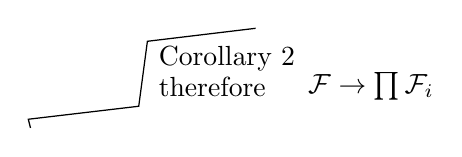
\begin{tikzpicture}[x=0.55cm,y=0.55cm]
\draw[line width=0.45pt] (-2.5,-1.4) -- (-2.55,-1.2) -- (0,-0.9) -- (0.2,0.6) -- (2.7,0.9);
\node[anchor=west,inner sep=0pt] at (0.45,0.2) {\inserted{\uline{Corollary 2}}};
\node[anchor=west,inner sep=0pt] at (0.45,-0.45) {\deleted{\unsure{therefore}}};
\node[anchor=west,inner sep=0pt] at (3.9,-0.45) {$\mathcal F\to\prod\mathcal F_i$};
\end{tikzpicture}}
is a bijection in \unsure{the\deleted{s}|the} \deleted{two} case where \deleted{following} \inserted{$I$ is finite.}

\deleted{a) $I$ is finite}

\deleted{b) Every figure is of finite type -- then}

\uline{Corollary 3} Suppose that the figures \deleted{\unsure{of|of the}} $\in\mathcal F$ are of finite type \deleted{Then it} \inserted{(resp. finite)}. Then the same holds \deleted{\unsure{of}} for $\mathcal F_i$, moreover $\mathcal F\unsure{\text{---}|\longrightarrow}\prod\mathcal F_i$ has as image the set of $(F_i)$ such that $F_i$ is $\varnothing$ for \unsure{al|al|al}most every $i$.
